\documentclass[10pt,twocolumn]{article}
\usepackage{graphicx}
\usepackage{amssymb}
\usepackage{titling}
\usepackage{url,hyperref}

\begin{document}

\title{Detecting Fraudulent Universities}

\author{Michelle Ho and Shay Lehmann}

\date{%
CUSP-GX-5006\\
Machine Learning Final Project \\
\rule{\textwidth}{1pt}
}

\posttitle{\par\rule{3in}{0.4pt}\end{center}\vskip 0.5em}
%\postdate{\rule{\textwidth}{1pt}}

\maketitle

\begin{abstract}

For this project, the authors sought to examine higher education in the United States
using the College Scorecard dataset. Their goals were twofold: 1) predict cohort's 3-year
default rate based on information about the institution and 2) proactively identify
potentially fraudulent schools.

\end{abstract}


\section{Introduction}

In the United States, the rising cost of a college degree and the corresponding
increase in student loans is well-documented. Nonetheless, a college degree is the bare
minimum requirement for many positions regardless of whether the specific major
has provided any subject matter expertise relevant to the industry. The authors
initially set out to identify the 'best value' colleges and chose the rate of
student loan default on federally-funded loans as the metric with which to define
value. Since most defaults are the result of a borrower being unable to make monthly
payments, a default suggests that the student did not obtain a well-paying position.
Furthermore, the default will negatively affect credit history for years to come. Exploratory analysis
revealed significant discrepancies in the distribution of loan default by
institution type (public, private not-for-profit and private for-profit), with public and
private not-for-profits exhibiting similar patterns. Private for-profit schools, on the other hand,
exhibited a significantly
higher mean default rate as well as a much larger range of potential outcomes with
some schools reaching default rates over 30\% (Figure~\ref{boxplot}).
The authors then
began a secondary inquiry to determine whether they could identify fraudulent or
potentially fraudulent universities. A number of for-profit universities that are part of
the Corinthian College network have recently come under investigation by the federal government
for their graduates' high default rates and misleading promises about job placement rates. In many instances,
the federal government has forgiven several millions of dollars in outstanding loans.
While loan forgiveness is one step towards aiding the victims, it does not
compensate them or remediate inadequate education.
The authors hope machine learning techniques can be used to identify a school's
3-year loan default rate and fraudulent schools in particular. They hope that this
will enable the government to take proactive steps towards investigating such universities
before they are able to embezzle years of federal funds while delivering low quality
education. The authors also hope that publicizing the high default rates will prompt
reform of the process and build support for increased funding for public universities.


\section{Methods and Data Sets}
This report makes use of the College Scorecard dataset. This dataset is relatively new
initiative to compile education-related from disparate federal institutions into
one centralized location from over the past 20 years.
Although the earliest cohorts were from the late 1990s, measurements have changed
over the years and many do not have data available for all variables.
As such, the authors examined data from the 2011-2013 cohorts in order to predict
the 3-year default rate for the cohort and 2010-2011 cohort for detecting fraudulent
schools. The College Scorecard dataset includes 7414 schools and 1743 variables on basic
identifying information, admissions, student body demographics, degree programs,
tuition costs, federal aid, debt repayment, completion rates, and earnings.
However, there is not complete coverage for all variables depending on the
institution. For the analyses in this paper, the data was subsetted based upon available
features.

For the first part of analysis (default rate prediction) the used variables are described below:

\begin{itemize}
\item \texttt{CONTROL}: a categorical variable indicating the funding type of a school.
Categories are 1=``public", 2=``private non-profit", or 3=``private for-profit".
\item \texttt{CDR3}: Cohort Default Rate at 3 Years
\item \texttt{MAIN}: Boolean identifier for main campus
\item \texttt{LO\char`_INC\char`_DEBT\char`_MDN}: The median debt for students with family income between \$0-\$30,000
\item \texttt{HI\char`_INC\char`_DEBT\char`_MDN}: The median debt for students with family income \$75,001+
\item \texttt{MD\char`_INC\char`_DEBT\char`_MDN}: The median debt for students with family income between \$30,001-\$75,000
\item \texttt{FIRST\char`_GEN}: Share of students who are first-generation students
\item \texttt{COMP\char`_ORIGIN\char`_YR4\char`_RT}:  Share of students who complete at the original university within 4 years
\item \texttt{ADM\char`_RATE\char`_ALL}: The admissions rate for the entire school
\item \texttt{AGE\char`_ENTRY}: The average age at time of entry for students
\item \texttt{INEXPFTE}: Dollars spent by the institution on education per full-time student
\item The dependent variable being classified and predicted is `CDR3' for the first step.
\item The data was limited to only the main campus for each institution as many features
were reported as identical for each satellite campus leading to redundant entries.
The MAIN column was then dropped for further analysis.
\item The independent variables are all the others.
\item Any observations with null values for any of the chosen variables
are dropped. After these drops, the number of observations
in the dataset is 2122 for the 2011 cohort, 2151 for the 2012 cohort, 2052 for the
2013 cohort.
\item Finally, the categorical variable \texttt{CONTROL} is binarized so that all samples
are represented by boolean feature vectors.
\end{itemize}


The steps taken for the default rate prediction were:
\begin{enumerate}
\item Random Forest Regression is run on the 2011 cohort using test sizes (as fraction of data) of .25, .33,
.5, .67 and .75 with a depth of 8 and the resulting in- and out-of-sample $R^2$
visualized (Figure~\ref{Testsize}).
\item Random Forest Regression is run on the 2011 cohort using depths ranging from 3-11 and the
resulting in- and out-of-sample $R^2$ visualized (Figure~\ref{maxdepth}).
\item Random Forest Regressions are run on each cohort with a test size of .33, a
max depth of 8 and 100 trees in the forest. Resulting actual v. predicted are visualized for both test and training samples
(Figure~\ref{results2011}, Figure~\ref{results2012}, Figure~\ref{results2013})
\item Random Forest Regression is run using the 2011 cohort as training set and the
2013 cohort as test set (Figure~\ref{2013from2011}).
\item Data from the 2011 and 2012 cohorts are grouped by school and averaged if the
school was in both cohorts. Random Forest Regression is run on the averaged data and used to
predict the 3-year default rate for the 2013 cohort (Figure~\ref{2013blended})
\end{enumerate}

Variables used for the the second part of analysis (fraudulent school detection):

\begin{itemize}

\item 38 float variables on program degree breakdown (ie. \% of degrees awarded in Architecture)
\item 13 float variables on undergraduate demographics (ie. \% of certain race, \% of certain gender)
\item 2 variables on default rate \texttt{CDR2}, the two year default rate, and \texttt{CDR2\char`_DENOM},
the number of students used to calculate the two year default rate
\item 16 categorical variables on school type (region of location, \texttt{CONTROL}, four-year or two-year school)
\item 1 binary variable serving as a label for a Corinthian school or not (independent variable).
This variable, not part of the College Scorecard dataset, was created by finding all school
names that started with `Heald`, `Everest`, or `WyoTech` (all schools in the Corinthian school network)
and labeling them witn `1`.
\item The dependent variable being predicted is the Corinthian label.
\item The independent variables are all the others.
\item All columns that contained null values or Privacy Suppressed values for
any Corinthian schools were dropped
\item Any rows that contained null values or Privacy Suppressed for those columns were dropped
\item Finally, the categorical variables are binarized so that all samples
are represented by boolean feature vectors
\item The number of observations in the dataset is 5486 schools and 70 variables
\end{itemize}

The methodology for classification of Corinthian schools:
\begin{enumerate}
\item Three classification models were tested: Logistic Regression, Support Vector Machines (SVM).
and Naive Bayes. All models were implemented using
modules from the Python package sci-kit learn.
\item All models were tested using cross validation method, with the dataset
split into training and test sets at 80\% and 20\%, respectively.
\item All models were fit with the training data and used to predict on the test set,
and accuracy was assessed by comparing misclassified predictions across models.
\item For the Logistic model, a numerical assessment was conducted for changes in accuracy
with changes in the class\char`_weight parameter. Although a class\char`_weight between 0.2 and 0.4 yielded the highest
overall accuracy (Figure~\ref{accuracy}), no Corinthian schools were correctly classified with class\char`_weight 0.2, as every school
was classified as non-Corinthian (Figure~\ref{log_unbalanced}). As such, class\char`_weight
was ultimately set to 'balanced' to automatically adjust
weights of the error terms inversely proportional to class frequencies in the input data (Figure~\ref{log_balanced}).
\item For the SVM model, the class\char`_weight parameter was also set to 'balanced', and a
linear kernel was used to fit the model (Figure~\ref{SVM_balanced})
\item The Naive Bayes classifier was fit with a Bernoulli distribution (Figure~\ref{naive_bayes})
\item Confusion matrices were generated for the balanced models to evaluate accuracy.
\item Finally, an unsupervised learning method was attempted using peer group analysis. Each
school was compared with its k-nearest neighbors on the chosen metric, 2-year default rate.
Schools that were one standard deviation above average in default rate were flagged as potentially fraudulent schools.
\item The k-nearest neighbors approach was implemented in sci-kit learn and used only normalized
variables of the 70 variables used in the earlier classification models. In other words, categorical
variables were removed and all variables were float values between 0 and 1.
\item Varying neighborhood sizes were tested between 10 and 50
\end{enumerate}


\section{Results}

For the default rate prediction analysis, the two preliminary examinations of tree depth and test size were used to set the
test size and max depth for the remainder of tests. In-sample $R^2$ was robust against test
 size, but out-of-sample $R^2$ was much more sensitive. With regard to the depths,
in-sample $R^2$ and out-of-sample $R^2$ increased for both with more steps. However,
out-of-sample plateaued at 8. Therefore, a test size of .33 and a maximum depth of 8 were
used for subsequent models.

Models were then trained within each cohort. The model trained on the 2011 cohort data
had an in sample $R^2 = .928$ and an out-of-sample $R^2 = .802$. The most important
features based on percentage of models in which they occurred were \texttt{FIRST\char`_GEN} (53.2\%),
\texttt{MD\char`_INC\char`_DEBT\char`_MDN} (12.3\%) and \texttt{COMP\char`_ORIG\char`_YR4\char`_RT} (10.8\%).
The model trained on the 2012 cohort data
had an in sample $R^2 = .929$ and an out-of-sample $R^2 = .826$. The most important
features based on percentage of models in which they occurred were \texttt{FIRST\char`_GEN} (55.7\%)
and \texttt{COMP\char`_ORIG\char`_YR4\char`_RT} (20.5\%). The model trained on the 2013 cohort data
had an in sample $R^2 = .915$ and an out-of-sample $R^2 = .772$. The most important
features based on percentage of models in which they occurred were
\texttt{COMP\char`_ORIG\char`_YR4\char`_RT} (46.1\%),
\texttt{FIRST\char`_GEN} (17.9\%) and CONTROL = Private For-Profit (15.8\%). Since Private For-Profit
institutions have such a wide range of default percentages as compared to the other two types,
the tree often split on other factors that are concentrated within high default rates, namely
a large share of first generation students and a low proportion who finish within four
years.

Given the variety from year to year, the authors attempted to validate a model
trained on 2011 data with results from 2013. However, this model lost some of its
predictive power with a wider spread, especially in the highest default rates.

Lastly, the authors attempted to improve upon this year to year model by by averaging
the features over years 2011 and 2012 in order to test 2013 data. This model did
not improve upon the previous model and exhibited the same loss of predictive capability,
particularly for the highest default rates.

The authors suspect that there may be additional factors that cause an exceptionally
high default rate that may be missing from either the model or the dataset. Additional
research into those schools which were greatly under-predicted may help to identify
those factors.

For the fraud detection classification analysis, it appeared that Naive Bayes performed
the best in classifying Corinthian schools. In the test set, all 13 schools were correctly
identified. 177 non-Corinthian schools were misclassified, but for the purposes of fraud
detection, this is a desirable trait. These 177 schools would serve as a good starting
point for investigation for potential fraud. The Logistic model performed the next best,
only missing one Corinthian school, and had fewer false positives for non-Corinthian schools.
The balanced SVM model the worst, missing 4 Corinthian schools, but also with fewer
false positives for non-Corinthian.

The peer group analysis performed poorly compared to the supervised models. When compared to 10 closest
neighbors, 896 schools out of 5486 were flagged as potentially fraudulent. 42
true positives (Corinthian schools) were not flagged. The reasoning for this is that
Corinthian schools are more likely to be neighbors with each other, and therefore will
have a higher neighborhood average in 2-year default rate. The maximum CDR2 for
Corinthian schools was 0.315 and average was 0.214. The global mean was 0.09. To mitigate this,
the neighborhood size was increased incrementally to 50 schools. The number of flagged schools
fluctuated with a downward trend, but the number of missed Corinthian schools decreased with larger
neighborhood size (Figure~\ref{peer_group} and Figure~\ref{peer_group2}).

Python code used to generate the results, tables, and figures for this project can be
found at \url{https://github.com/michellemho/machine_learning_for_cities}.


\begin{figure*}[!t]
  \begin{center}
    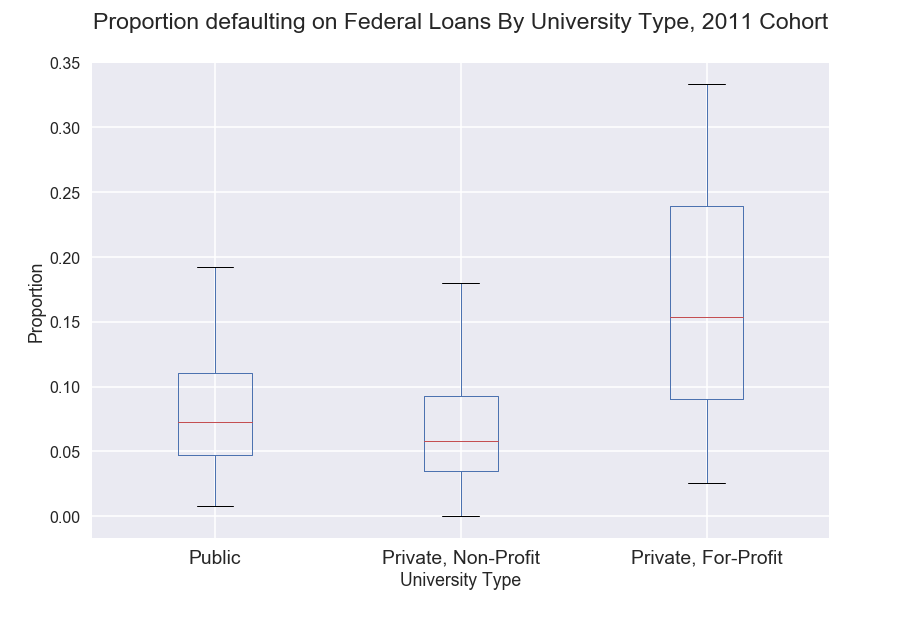
\includegraphics[width=\textwidth]{fedloans.png}
  \end{center}

  \caption{\Figure Exploratory look at difference between default rates by Control Group, 2011}
  \label{boxplot}
\end{figure*}

\begin{figure*}[!t]
  \begin{center}
    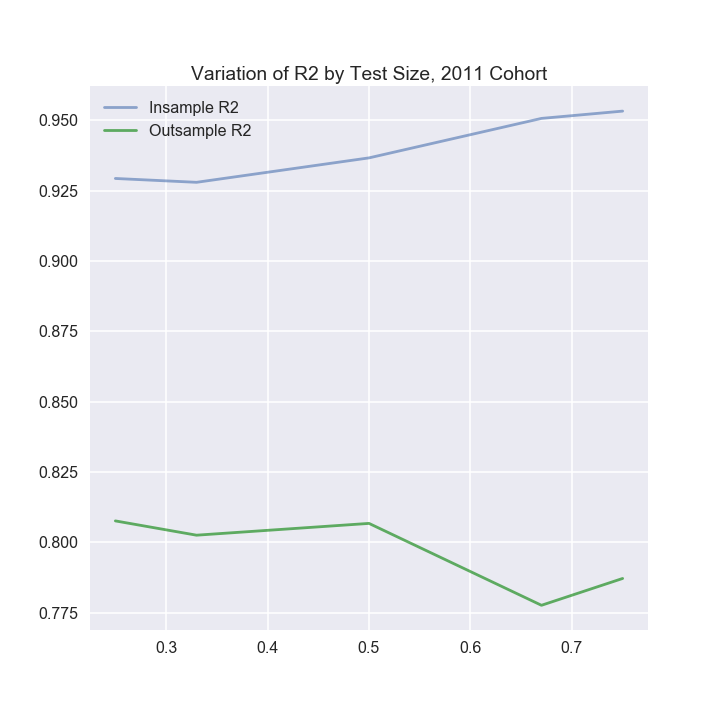
\includegraphics[width=\textwidth]{Testsize.png}
  \end{center}

  \caption{\Figure Exploration of Effect of Test Size on Random Forest Regression, 2011 Cohort}
  \label{Testsize}
\end{figure*}

\begin{figure*}[!t]
  \begin{center}
    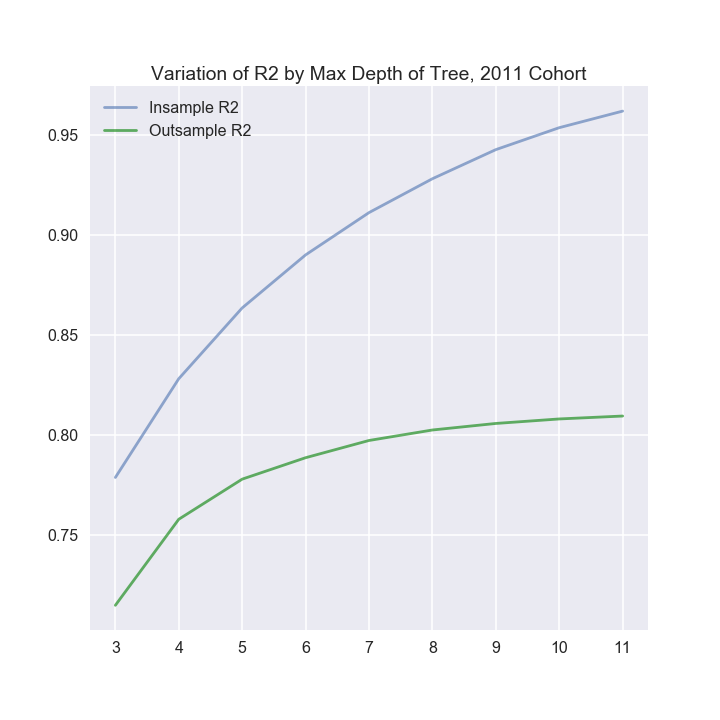
\includegraphics[width=\textwidth]{Max_Depth.png}
  \end{center}

  \caption{\Figure Exploration of Effect of Max Depth on Random Forest Regression, 2011 Cohort}
  \label{maxdepth}
\end{figure*}

\begin{figure*}[!t]
  \begin{center}
    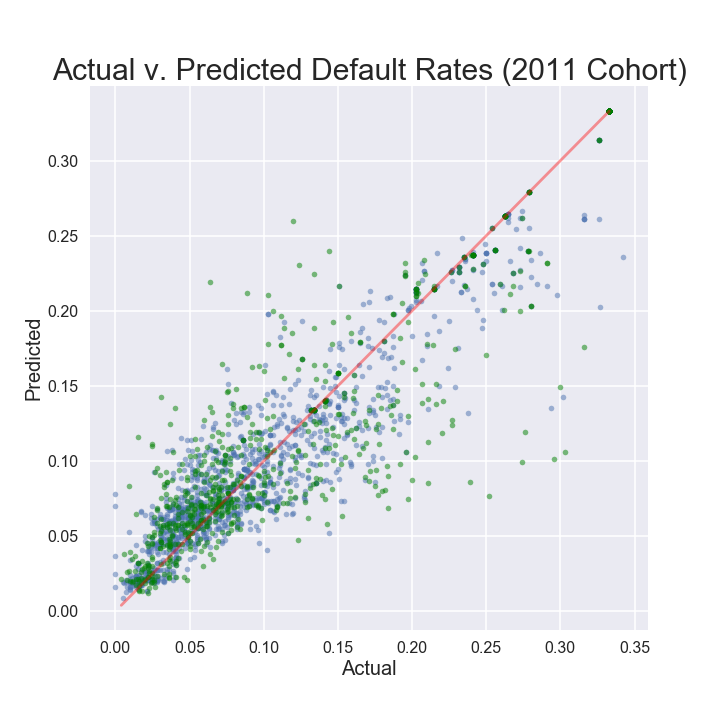
\includegraphics[width=\textwidth]{results2011.png}
  \end{center}

  \caption{\Figure Results of the model trained on data from the 2011 cohort}
  \label{results2011}
\end{figure*}

\begin{figure*}[!t]
  \begin{center}
    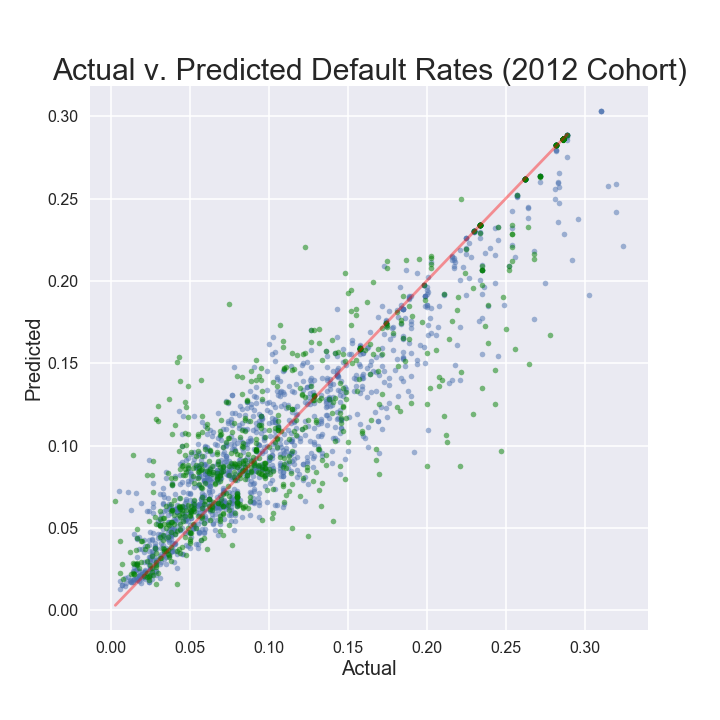
\includegraphics[width=\textwidth]{results2012.png}
  \end{center}

  \caption{\Figure Results of the model trained on data from the 2012 cohort}
  \label{results2012}
\end{figure*}

\begin{figure*}[!t]
  \begin{center}
    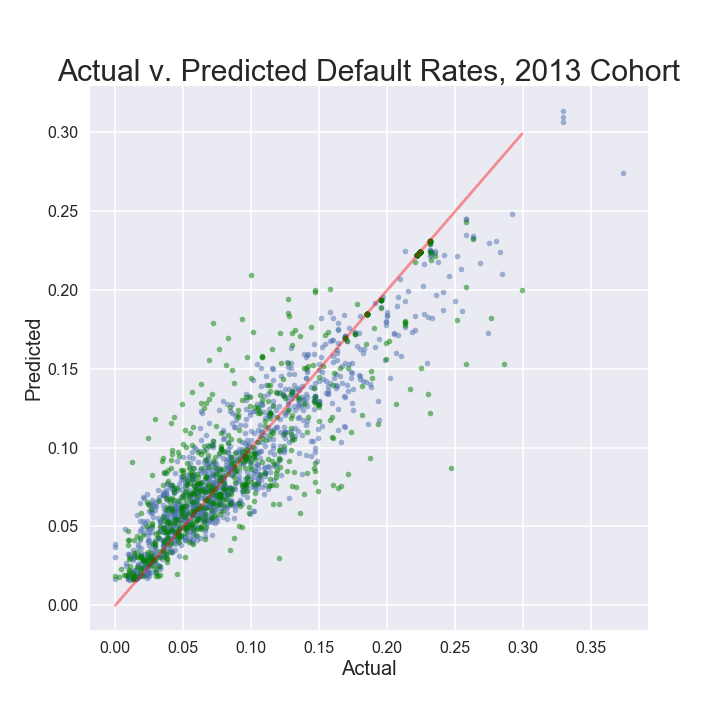
\includegraphics[width=\textwidth]{results2013.png}
  \end{center}

  \caption{\Figure Results of the model trained on data from the 2013 cohort}
  \label{results2013}
\end{figure*}

\begin{figure*}[!t]
  \begin{center}
    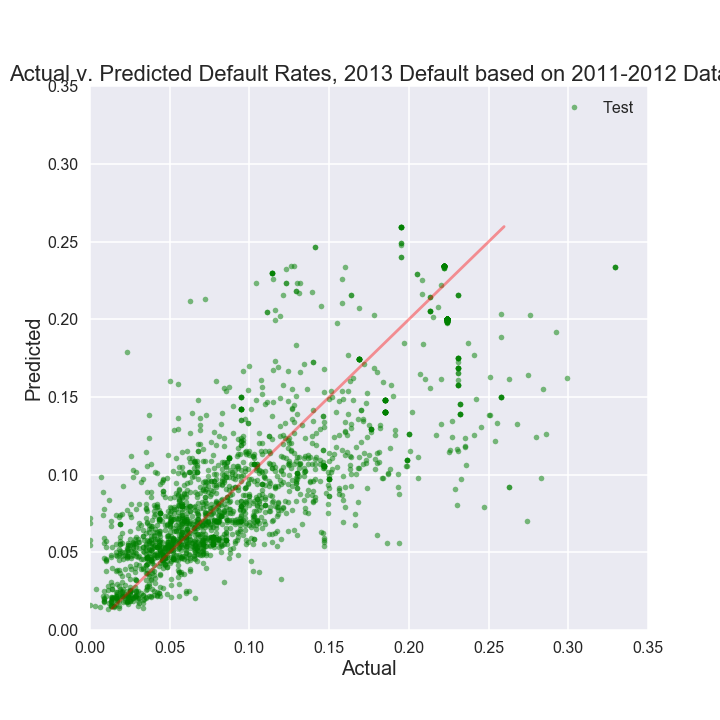
\includegraphics[width=\textwidth]{2013from2011.png}
  \end{center}

  \caption{\Figure Results of the model trained on data from the 2011 cohort
  and tested on the 2013 cohort}
  \label{2013from2011}
\end{figure*}

\begin{figure*}[!t]
  \begin{center}
    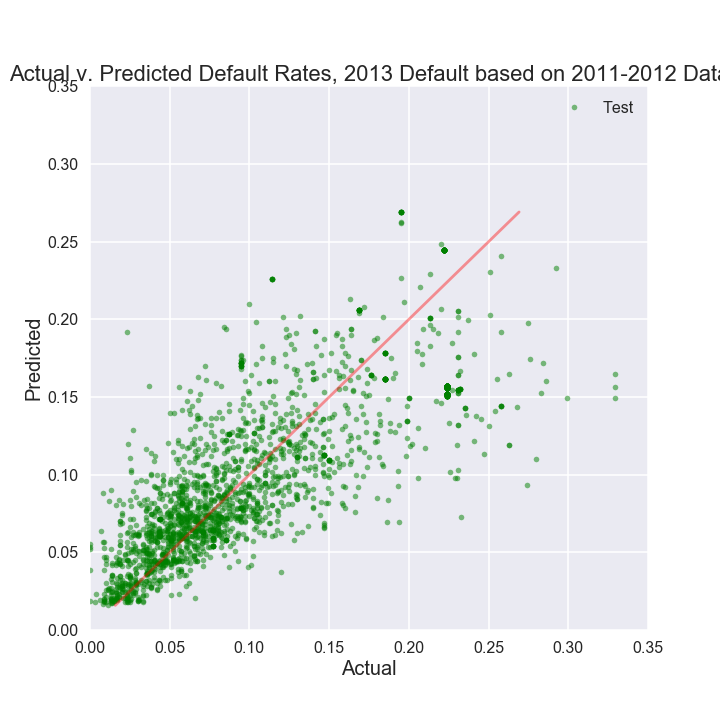
\includegraphics[width=\textwidth]{2013blended.png}
  \end{center}

  \caption{\Figure Results of the model trained on averaged data from 2011-2012 cohorts
  and tested on the 2013 cohort}
  \label{2013blended}
\end{figure*}

\begin{figure*}[!t]
  \begin{center}
    \includegraphics[width=\textwidth]{Accuracy_Logistic.png}
  \end{center}

  \caption{\Figure Results of the logistic model at varying class weights}
  \label{accuracy}
\end{figure*}


\begin{figure*}[!t]
  \begin{center}
    \includegraphics[width=\textwidth]{logreg_classweight02.png}
  \end{center}

  \caption{\Figure Results of the logistic model at class weight = 0.2}
  \label{log_unbalanced}
\end{figure*}

\begin{figure*}[!t]
  \begin{center}
    \includegraphics[width=\textwidth]{Logistic_Balanced.png}
  \end{center}

  \caption{\Figure Results of the balanced logistic model}
  \label{log_balanced}
\end{figure*}

\begin{figure*}[!t]
  \begin{center}
    \includegraphics[width=\textwidth]{SVM_linear_balanced.png}
  \end{center}

  \caption{\Figure Results of the balanced SVM Linear model}
  \label{SVM_balanced}
\end{figure*}

\begin{figure*}[!t]
  \begin{center}
    \includegraphics[width=\textwidth]{Naive Bayes.png}
  \end{center}

  \caption{\Figure Results of the Naive Bayes model}
  \label{naive_bayes}
\end{figure*}

\begin{figure*}[!t]
  \begin{center}
    \includegraphics[width=\textwidth]{flaggedfraud.png}
  \end{center}

  \caption{\Figure Results of the Peer Group Analysis}
  \label{peer_group}
\end{figure*}

\begin{figure*}[!t]
  \begin{center}
    \includegraphics[width=\textwidth]{missed_corin.png}
  \end{center}

  \caption{\Figure Results of the peer group analysis in detecting Corinthian Schools}
  \label{peer_group2}
\end{figure*}




\end{document}
